\documentclass[
  12pt,
  a4paper,
  DIV=12,
  spanish,
]{scrartcl}

\linespread{1.3}
\setlength{\parindent}{0pt}
\setlength{\parskip}{1em}

\usepackage{babel}

%% Fuentes personalizadas para utilizar con XeTeX
\usepackage{unicode-math}
\setmainfont[
  Path = ./fonts/,
  UprightFont = *-Regular,
  ItalicFont = *-Italic,
  BoldFont = *-Bold,
  BoldItalicFont = *-BoldItalic,
]{FiraSans}
\setsansfont[
  Path = ./fonts/,
  UprightFont = *-Regular,
  ItalicFont = *-Italic,
  BoldFont = *-Bold,
  BoldItalicFont = *-BoldItalic,
]{FiraSans}
\setmathfont[
  Path = ./fonts/,
]{FiraMath-Regular}
\setmathfont[
  range={it/{latin, Latin}},
  math-style=TeX,
  Path = ./fonts/,
]{FiraSans-Italic}

\usepackage[activate={true,nocompatibility},final,tracking=true,factor=1100,stretch=10,shrink=10]{microtype}
\SetTracking{encoding={*}, shape=sc}{0}

\usepackage{enumitem}
\setlist[itemize]{leftmargin=*, noitemsep, topsep=0pt}
\setlist[enumerate]{leftmargin=*}

\usepackage{changepage}

%% estos creo que no los usados... los dejo por si acaso
\newcommand{\term}[2]{\textbf{#1}\quad#2\\}
\newcounter{ObjCounter}
\newcommand{\obj}[1]{\addtocounter{ObjCounter}{1}\textbf{\rmfamily OBJ-\theObjCounter}\quad#1\\}

% Contadores requisitos funcionales fs
\newcounter{RF}
\setcounter{RF}{1}
\newcounter{RFu}[RF]
\setcounter{RFu}{0}
\renewcommand{\theRFu}{\theRF.\arabic{RFu}}
\newcommand{\rfu}[1]{\noindent%
  \refstepcounter{RFu}\textbf{RF \theRFu}\quad #1\\%
}
\newcounter{RFd}[RF]
\setcounter{RFd}{0}
\renewcommand{\theRFd}{\theRF.\arabic{RFd}}
\newcommand{\rfd}[1]{\noindent%
  \refstepcounter{RFd}\textbf{RF \theRFd}\quad #1\\%
}
\newcounter{RFt}[RF]
\setcounter{RFt}{0}
\renewcommand{\theRFt}{\theRF.\arabic{RFt}}
\newcommand{\rft}[1]{\noindent%
  \refstepcounter{RFt}\textbf{RF \theRFt}\quad #1\\%
}
\newcounter{RFc}[RF]
\setcounter{RFc}{0}
\renewcommand{\theRFc}{\theRF.\arabic{RFc}}
\newcommand{\rfc}[1]{\noindent%
  \refstepcounter{RFc}\textbf{RF \theRFc}\quad #1\\%
}


% Contadores requisitos de datos
\newcounter{RD}
\setcounter{RD}{1}
\newcounter{RDu}
\setcounter{RDu}{0}
\renewcommand{\theRDu}{\theRD.\arabic{RDu}}
\newcommand{\rdu}[1]{\noindent%
  \refstepcounter{RDu}\textbf{RD \theRDu}\quad #1%
}
\newcounter{RDd}
\setcounter{RDd}{0}
\renewcommand{\theRDd}{\theRD.\arabic{RDd}}
\newcommand{\rdd}[1]{\noindent%
  \refstepcounter{RDd}\textbf{RD \theRDd}\quad #1%
}
\newcounter{RDt}
\setcounter{RDt}{0}
\renewcommand{\theRDt}{\theRD.\arabic{RDt}}
\newcommand{\rdt}[1]{\noindent%
  \refstepcounter{RDt}\textbf{RD \theRDt}\quad #1%
}
\newcounter{RDc}
\setcounter{RDc}{0}
\renewcommand{\theRDc}{\theRD.\arabic{RDc}}
\newcommand{\rdc}[1]{\noindent%
  \refstepcounter{RDc}\textbf{RD \theRDc}\quad #1%
}

% Contadores restricciones semánticas
\newcounter{RS}
\setcounter{RS}{1}
\newcounter{RSu}[RS]
\setcounter{RSu}{0}
\renewcommand{\theRSu}{\theRS.\arabic{RSu}}
\newcommand{\rsu}[1]{\noindent%
  \refstepcounter{RSu}\textbf{RS \theRSu}\quad #1%
}
\newcounter{RSd}[RS]
\setcounter{RSd}{0}
\renewcommand{\theRSd}{\theRS.\arabic{RSd}}
\newcommand{\rsd}[1]{\noindent%
  \refstepcounter{RSd}\textbf{RS \theRSd}\quad #1%
}
\newcounter{RSt}[RS]
\setcounter{RSt}{0}
\renewcommand{\theRSt}{\theRS.\arabic{RSt}}
\newcommand{\rst}[1]{\noindent%
  \refstepcounter{RSt}\textbf{RS \theRSt}\quad #1%
}
\newcounter{RSc}[RS]
\setcounter{RSc}{0}
\renewcommand{\theRSc}{\theRS.\arabic{RSc}}
\newcommand{\rsc}[1]{\noindent%
  \refstepcounter{RSc}\textbf{RS \theRSc}\quad #1%
}



\usepackage{array}
\usepackage{adjustbox}
\usepackage{tabularx}
\usepackage{ltablex}
\usepackage{float}

\title{Práctica DDSI}
\author{José María Martín Luque (Canciones) \and Luis Antonio Ortega Andrés (Usuarios) \and Sofía Almeida Bruno (Social) \and Antonio Martín Ruiz (Búsqueda)  }

\begin{document}

\maketitle
%% Índice
{\parskip=2pt
  \tableofcontents
}
\pagebreak

\section{Descripción del sistema y especificación de requisitos}

\documentclass[
  12pt,
  a4paper,
  DIV=12,
  spanish,
]{scrartcl}

\linespread{1.3}
\setlength{\parindent}{0pt}
\setlength{\parskip}{1em}

\usepackage{babel}

%% Fuentes personalizadas para utilizar con XeTeX
\usepackage{unicode-math}
\setmainfont[
  Path = ./fonts/,
  UprightFont = *-Regular,
  ItalicFont = *-Italic,
  BoldFont = *-Bold,
  BoldItalicFont = *-BoldItalic,
]{FiraSans}
\setsansfont[
  Path = ./fonts/,
  UprightFont = *-Regular,
  ItalicFont = *-Italic,
  BoldFont = *-Bold,
  BoldItalicFont = *-BoldItalic,
]{FiraSans}
\setmathfont[
  Path = ./fonts/,
]{FiraMath-Regular}
\setmathfont[
  range={it/{latin, Latin}},
  math-style=TeX,
  Path = ./fonts/,
]{FiraSans-Italic}

\usepackage[activate={true,nocompatibility},final,tracking=true,factor=1100,stretch=10,shrink=10]{microtype}
\SetTracking{encoding={*}, shape=sc}{0}

\usepackage{enumitem}
\setlist[itemize]{leftmargin=*, noitemsep, topsep=0pt}
\setlist[enumerate]{leftmargin=*}

\usepackage{changepage}

%% estos creo que no los usados... los dejo por si acaso
\newcommand{\term}[2]{\textbf{#1}\quad#2\\}
\newcounter{ObjCounter}
\newcommand{\obj}[1]{\addtocounter{ObjCounter}{1}\textbf{\rmfamily OBJ-\theObjCounter}\quad#1\\}

% Contadores requisitos funcionales fs
\newcounter{RF}
\setcounter{RF}{1}
\newcounter{RFu}[RF]
\setcounter{RFu}{0}
\renewcommand{\theRFu}{\theRF.\arabic{RFu}}
\newcommand{\rfu}[1]{\noindent%
  \refstepcounter{RFu}\textbf{RF \theRFu}\quad #1\\%
}
\newcounter{RFd}[RF]
\setcounter{RFd}{0}
\renewcommand{\theRFd}{\theRF.\arabic{RFd}}
\newcommand{\rfd}[1]{\noindent%
  \refstepcounter{RFd}\textbf{RF \theRFd}\quad #1\\%
}
\newcounter{RFt}[RF]
\setcounter{RFt}{0}
\renewcommand{\theRFt}{\theRF.\arabic{RFt}}
\newcommand{\rft}[1]{\noindent%
  \refstepcounter{RFt}\textbf{RF \theRFt}\quad #1\\%
}
\newcounter{RFc}[RF]
\setcounter{RFc}{0}
\renewcommand{\theRFc}{\theRF.\arabic{RFc}}
\newcommand{\rfc}[1]{\noindent%
  \refstepcounter{RFc}\textbf{RF \theRFc}\quad #1\\%
}


% Contadores requisitos de datos
\newcounter{RD}
\setcounter{RD}{1}
\newcounter{RDu}
\setcounter{RDu}{0}
\renewcommand{\theRDu}{\theRD.\arabic{RDu}}
\newcommand{\rdu}[1]{\noindent%
  \refstepcounter{RDu}\textbf{RD \theRDu}\quad #1%
}
\newcounter{RDd}
\setcounter{RDd}{0}
\renewcommand{\theRDd}{\theRD.\arabic{RDd}}
\newcommand{\rdd}[1]{\noindent%
  \refstepcounter{RDd}\textbf{RD \theRDd}\quad #1%
}
\newcounter{RDt}
\setcounter{RDt}{0}
\renewcommand{\theRDt}{\theRD.\arabic{RDt}}
\newcommand{\rdt}[1]{\noindent%
  \refstepcounter{RDt}\textbf{RD \theRDt}\quad #1%
}
\newcounter{RDc}
\setcounter{RDc}{0}
\renewcommand{\theRDc}{\theRD.\arabic{RDc}}
\newcommand{\rdc}[1]{\noindent%
  \refstepcounter{RDc}\textbf{RD \theRDc}\quad #1%
}

% Contadores restricciones semánticas
\newcounter{RS}
\setcounter{RS}{1}
\newcounter{RSu}[RS]
\setcounter{RSu}{0}
\renewcommand{\theRSu}{\theRS.\arabic{RSu}}
\newcommand{\rsu}[1]{\noindent%
  \refstepcounter{RSu}\textbf{RS \theRSu}\quad #1%
}
\newcounter{RSd}[RS]
\setcounter{RSd}{0}
\renewcommand{\theRSd}{\theRS.\arabic{RSd}}
\newcommand{\rsd}[1]{\noindent%
  \refstepcounter{RSd}\textbf{RS \theRSd}\quad #1%
}
\newcounter{RSt}[RS]
\setcounter{RSt}{0}
\renewcommand{\theRSt}{\theRS.\arabic{RSt}}
\newcommand{\rst}[1]{\noindent%
  \refstepcounter{RSt}\textbf{RS \theRSt}\quad #1%
}
\newcounter{RSc}[RS]
\setcounter{RSc}{0}
\renewcommand{\theRSc}{\theRS.\arabic{RSc}}
\newcommand{\rsc}[1]{\noindent%
  \refstepcounter{RSc}\textbf{RS \theRSc}\quad #1%
}



\usepackage{array}
\usepackage{adjustbox}
\usepackage{tabularx}
\usepackage{ltablex}

\title{Práctica 1. Descripción del sistema y especificación de requisitos \\\large Diseño y Desarrollo de Sistemas de Información}
\author{Sofía Almedia Bruno \and José María Martín Luque \and Antonio Martín Ruiz \and Luis Antonio Ortega Andrés}

\begin{document}

\maketitle

\section{Descripción del sistema} % (fold)

El sistema es una red social para gestionar y compartir opiniones sobre música. Incluye un registro de la música que el usuario ha escuchado así como un sistema de sugerencias generadas a partir de sus escuchas y las de las personas a las que sigue.

%%Subsistema de música
Se pueden consultar y añadir tanto canciones como autores y géneros.

Para incorporar una canción es necesario especificar título (en una serie de hasta 50 caracteres), autor o autores de los preexistentes y género de entre los preexistentes. Adicionalmente se podrán completar estos datos con la fecha de lanzamiento (8 números en formato de fecha dd/mm/aaaa), álbum al que pertenece (serie de hasta 20 caracteres) o portada (imagen PNG de dimensiones 512 $\times$ 512). El sistema generará un identificador único para cada canción (como un número de 16 dígitos).

Para agregar un autor es necesario especificar su nombre (una lista en la cual cada elemento es una serie de hasta 30 caracteres), y adicionalmente se puede indicar su procedencia (ciudad y país, como una lista de 20 caracteres cada uno), intervalo de actividad (dos fechas en el formato previamente especificado, siendo la segunda sustituible por ``Actualidad''), fotografía (imagen PNG) y una biografía (en una serie de hasta 2000 caracteres) y géneros relacionados de entre los preexistentes. El sistema generará un identificador único para cada autor (como un número de 16 dígitos).

Para agregar un género musical solo es necesario introducir un nombre (como una cadena de hasta 20 caracteres). Adicionalmente se puede añadir una breve descripción (como una cadena de hasta 500 caracteres).

Cualquiera de estos datos pueden ser modificados o eliminados por un usuario con los permisos adecuados, excepto los identificadores de las canciones y los autores que solo podrán ser eliminados al eliminar la canción o autor correspondiente.

%%Subsistema de usuarios

Para añadir un nuevo usuario al sistema es imprescindible indicar nombre de usuario (una serie de hasta 12 caracteres, que funcionará como identificador, luego debe ser único) y una contraseña (una serie de entre 7 y 128 caracteres). Además, se puede indicar un correo electrónico (con formato estándar), una biografía (como una serie de hasta 500 caracteres) y una fotografía (imagen PNG).

Existen tres tipos de usuario según sus permisos. Los administradores pueden añadir, editar y eliminar cualquier elemento de la base de datos. Los moderadores se encargan de añadir, modificar y borrar canciones, autores y géneros. Su función es mantener el sistema actualizado y correcto. Los usuarios por defecto solo pueden modificar su propio perfil. Al crear un nuevo usuario, este será por defecto. Un administrador puede convertir a un usuario por defecto en moderador o administrador.

Cada usuario tiene asociado un perfil en el que se mostrarán las canciones que el usuario ha marcado como escuchadas así como sus valoraciones, comentarios y canciones favoritas.

%%Subsistema social

Cualquier usuario puede marcar una canción como escuchada, como pendiente o como favorita, añadir una valoración (un valor entero entre 0 y 10) y un comentario (una serie de hasta 500 caracteres). Para marcar como favorita, añadir una valoración o un comentario, primero habrá que haber marcado como escuchada esa canción.

Un usuario puede seguir a otro usuario, teniendo así una notificación de cuándo el usuario al que sigue realiza alguna actividad. Las sugerencias de búsqueda se verán también influidas por los usuarios a los que se sigue.


%%Subsistema de búsqueda

Se pueden buscar canciones en el sistema por su título, autor, género, álbum o año. También pueden consultarse autores y géneros, de los cuales se podrá obtener la información que exista en el sistema y una lista de canciones relacionadas.

Existe un sistema de sugerencias consistente en búsquedas programadas automáticamente en función de las canciones que un usuario y sus seguidos hayan añadido a favoritos y valorado, teniendo en cuenta la puntuación dada.

\section{Requisitos de datos}
\subsection{Datos de entrada}

% Música

\rdu{Datos utilizados al añadir una nueva canción \label{rdu:datos-nueva-cancion}}
\begin{itemize}
  \item Título (Una cadena no vacía de hasta 50 caracteres)
  \item Fecha (8 números en formado dd/mm/aaaa)
  \item Autor (Identificador del autor)
  \item Género (Nombre del género, cadena de hasta 20 caracteres)
  \item Álbum (Serie de hasta 20 caracteres)
  \item Portada (opcional) (Imagen PNG de dimensiones 512x512)
  \item Identificador (Cadena de 16 caracteres numéricos)
\end{itemize}

\rdu{Datos utilizados al añadir un nuevo género \label{rdu:datos-nuevo-genero}}
\begin{itemize}
  \item Nombre (Cadena de hasta 20 caracteres)
  \item Descripción (Cadena de hasta 500 caracteres)
\end{itemize}

\rdu{Datos utilizados al añadir un nuevo autor\label{rdu:datos-nuevo-autor}}

\begin{itemize}
  \item Nombre (Cadena de hasta 30 caracteres)
  \item Procedencia (opcional) (Dos listas de 20 caracteres alfanuméricos)
  \item Intervalo de actividad (opcional) (Dos fechas en el formato dd/mm/aaaa, siendo la segunda sustituible por ``actualidad'') (opcional)
  \item Foto (opcional) (Imagen en formato PNG)
  \item Biografía (opcional) (Serie de hasta 2000 caracteres alfanuméricos)
    \item Géneros relacionados (opcional) (Lista de nombres de géneros)
    \item Identificador de un autor (cadena numérica de 16 caracteres)
\end{itemize}

\refstepcounter{RD}

% Usuario

\rdd{Datos utilizados en el registro de un nuevo usuario\label{rdd:registro-usuario}}
\begin{itemize}
\item Alias (Una serie de hasta 12 caracteres)
\item Contraseña (Una serie de entre 7 y 128 caracteres).
\item Correo electrónico (opcional) (Serie de caracteres en formato xxxxx@yyyy.zzz)
\item Fecha de nacimiento (opcional) (Serie de caracteres en formato dd/mm/aaaa)
\item Foto (opcional) (Imagen en formato PNG)
\item Biografía (opcional) (Serie de hasta 500 caracteres)
\end{itemize}
\rdd{Datos de inicio de sesión \label{rdd:inicio-sesion}}
\begin{itemize}
\item Alias (Una serie de hasta 12 caracteres)
\item Contraseña (Una serie de entre 7 y 128 caracteres)
\end{itemize}
\rdd{Datos introducidos para la modificación de un dato personal\label{rdd:modificar-dato}}
\begin{itemize}
\item Alias (Una serie de hasta 12 caracteres)
\item Contraseña (Una serie de entre 7 y 128 caracteres)
\item Dato antiguo (En el formato correspondiente al dato)
\item Dato nuevo (En el mismo formato que el dato eliminado)
\end{itemize}
\rdd{Datos de autenticación para la baja de un usuario \label{rdd:inicio-sesion-baja}}
\begin{itemize}
\item Alias (Una serie de hasta 12 caracteres)
\item Contraseña (Una serie de entre 7 y 128 caracteres)
\end{itemize}
\rdd{Datos introducidos para acceder al perfil de un usuario \label{rdd:ver-perfil}}
\begin{itemize}
\item Alias del usuario (Serie de hasta 12 caracteres).
\end{itemize}
\refstepcounter{RD}

% Social - datos entrada
\rdt{Los datos para introducir un comentario\label{rdt:comentario-ent}}
\begin{itemize}
\item Alias de usuario (Una serie de hasta 12 caracteres del usuario que introduce el comentario)
\item Identificador de canción (Cadena de 16 caracteres numéricos)
\item Texto (Una cadena de hasta 500 caracteres no vacía)
\end{itemize}

\rdt{Los datos de una valoración\label{rdt:valoracion-ent}}
\begin{itemize}
\item Alias de usuario (Una serie de hasta 12 caracteres del usuario que introduce el comentario)
\item Identificador de canción (Cadena de 16 caracteres numéricos)
\item Valor (Un número entero entre 0 y 10)
\end{itemize}

\rdt{Los datos de las canciones escuchadas\label{rdt:escuchadas-ent}}
\begin{itemize}
\item Alias de usuario (Una serie de hasta 12 caracteres del usuario que introduce el comentario)
\item Identificador de canción (Cadena de 16 caracteres numéricos)
\end{itemize}

\rdt{Los datos de las canciones pendientes\label{rdt:pendientes-ent}}
\begin{itemize}
\item Alias de usuario (Una serie de hasta 12 caracteres del usuario que introduce el comentario)
\item Identificador de canción (Cadena de 16 caracteres numéricos)
\end{itemize}

\rdt{Los datos de las canciones favoritas\label{rdt:favoritas-ent}}
\begin{itemize}
\item Alias de usuario (Una serie de hasta 12 caracteres del usuario que introduce el comentario)
\item Identificador de canción (Cadena de 16 caracteres numéricos)
\end{itemize}

\rdt{Los datos para seguir a un usuario\label{rdt:seguir-ent}}
\begin{itemize}
\item Alias del usuario que sigue (Una serie de hasta 12 caracteres del usuario que sigue)
\item Alias del usuario que seguido (Una serie de hasta 12 caracteres del usuario seguido)
\end{itemize}

\rdt{Datos para ver información de una canción \label{rdt:id-cancion}}
\begin{itemize}
\item Identificador de una canción (Cadena de 16 caracteres numéricos)
\end{itemize}

\rdt{Datos para ver valoración \label{rdt:ver-val-ent}}
\begin{itemize}
\item Alias de usuario (una cadena de hasta 12 caracteres)
\item Identificador de una canción (Cadena de 16 caracteres numéricos)
\end{itemize}

\rdt{Datos para ver favoritos \label{rdt:ver-fav-ent}}
\begin{itemize}
\item Alias de usuario (una cadena de hasta 12 caracteres)
\end{itemize}

\rdt{Datos para ver pendientes \label{rdt:ver-pen-ent}}
\begin{itemize}
\item Alias de usuario (una cadena de hasta 12 caracteres)
\end{itemize}

\rdt{Datos para ver escuchadas \label{rdt:ver-esc-ent}}
\begin{itemize}
\item Alias de usuario (una cadena de hasta 12 caracteres)
\end{itemize}

\rdt{Datos para ver seguidos \label{rdt:ver-seguidos-ent}}
\begin{itemize}
\item Alias de usuario (una cadena de hasta 12 caracteres)
\end{itemize}

\refstepcounter{RD}

% Búsqueda

\rdc{Datos utilizados en una búsqueda\label{rdc:busqueda-ent}}
\begin{itemize}
\item Texto de la búsqueda (una cadena de entre 1 y 100 caracteres)
\end{itemize}


\subsection{Datos manejados}
\setcounter{RD}{1}

% Música
\rdu{Datos almacenados al añadir una nueva canción \label{rdu:datos-almacenados-nueva-cancion}}
\begin{itemize}
  \item Título (Una cadena no vacía de hasta 50 caracteres)
  \item Fecha (8 números en formado dd/mm/aaaa)
  \item Autor (Identificador del autor)
  \item Género (Nombre del género, cadena de hasta 20 caracteres)
  \item Álbum (Serie de hasta 20 caracteres)
  \item Portada (opcional) (Imagen PNG de dimensiones 512x512)
  \item Identificador (Cadena de 16 caracteres numéricos)
\end{itemize}

\rdu{Datos almacenados al añadir un nuevo género\label{rdu:datos-almacenados-nuevo-genero}}
\begin{itemize}
  \item Nombre (Cadena de hasta 20 caracteres)
  \item Descripción (Cadena de hasta 500 caracteres)
\end{itemize}

\rdu{Datos almacenados al añadir un nuevo autor\label{rdu:datos-almacenados-nuevo-autor}}

\begin{itemize}
  \item Nombre (Cadena de hasta 30 caracteres)
  \item Procedencia (opcional) (Dos listas de 20 caracteres alfanuméricos)
  \item Intervalo de actividad (opcional) (Dos fechas en el formato dd/mm/aaaa, siendo la segunda sustituible por `actualidad') (opcional)
  \item Foto (opcional) (Imagen en formato PNG)
  \item Biografía (opcional) (Serie de hasta 2000 caracteres alfanuméricos)
  \item Géneros relacionados (opcional) (Lista de nombres de géneros)
  \item Identificador de un autor (cadena numérica de 16 caracteres)
\end{itemize}


\refstepcounter{RD}

% Usuario
\rdd{Datos almacenados en el registro de un usuario\label{rdd:registro-usuario-almacenados}}
\begin{itemize}
  \item Alias (Una serie de hasta 12 caracteres)
  \item Contraseña (Una serie de entre 7 y 128 caracteres).
  \item Correo electrónico (opcional) (Serie de caracteres en formato xxxxx@yyyy.zzz)
  \item Fecha de nacimiento (opcional) (Serie de caracteres en formato dd/mm/aaaa)
  \item Foto (opcional) (Imagen en formato PNG)
  \item Biografía (opcional) (Serie de hasta 500 caracteres)
\end{itemize}

\rdd{Datos almacenados ante la modificación de un dato personal\label{rdd:modificar-dato-almacenados}}
\begin{itemize}
\item Dato modificado (En el formato correspondiente al dato)
\end{itemize}

\rdd{Datos eliminados ante la baja de un usuario \label{rdd:eliminar-usuario}}
\begin{itemize}
  \item Alias (Una serie de hasta 12 caracteres)
  \item Contraseña (Una serie de entre 7 y 128 caracteres).
  \item Correo electrónico (opcional) (Serie de caracteres en formato xxxxx@yyyy.zzz)
  \item Fecha de nacimiento (opcional) (Serie de caracteres en formato dd/mm/aaaa)
  \item Foto (opcional) (Imagen en formato PNG)
  \item Biografía (opcional) (Serie de hasta 500 caracteres)
\end{itemize}

\refstepcounter{RD}

% Social - datos manejados
\rdt{Los datos de un comentario almacenado\label{rdt:comentario-man}}
\begin{itemize}
\item Alias de usuario (Una serie de hasta 12 caracteres del usuario que introduce el comentario)
\item Identificador de canción (Cadena de 16 caracteres numéricos)
\item Texto (Una cadena de hasta 500 caracteres no vacía)
\end{itemize}

\rdt{Los datos de una valoración almacenada\label{rdt:valoracion-man}}
\begin{itemize}
\item Alias de usuario (Una serie de hasta 12 caracteres del usuario que introduce el comentario)
\item Identificador de canción (Cadena de 16 caracteres numéricos)
\item Valor (un número entero entre 0 y 10)
\end{itemize}

\rdt{Los datos almacenados de las canciones escuchadas\label{rdt:escuchadas-man}}
\begin{itemize}
\item Alias de usuario (Una serie de hasta 12 caracteres del usuario que introduce el comentario)
\item Identificador de canción (Cadena de 16 caracteres numéricos)
\item Escuchadas (lista formada por identificadores de canciones (Cadena de 16 caracteres numéricos))
\end{itemize}

\rdt{Los datos almacenados de las canciones pendientes\label{rdt:pendientes-man}}
\begin{itemize}
\item Alias de usuario (Una serie de hasta 12 caracteres del usuario que introduce el comentario)
\item Identificador de canción (Cadena de 16 caracteres numéricos)
\item Pendientes (lista formada por identificadores de canciones (Cadena de 16 caracteres numéricos))
\end{itemize}

\rdt{Los datos almacenados de las canciones favoritas\label{rdt:favoritas-man}}
\begin{itemize}
  \item Alias de usuario (Una serie de hasta 12 caracteres del usuario que introduce el comentario)
  \item Identificador de canción (Cadena de 16 caracteres numéricos)
  \item Favoritas (lista formada por identificadores de canciones (Cadena de 16 caracteres numéricos))
\end{itemize}

\rdt{Los datos de un usuario al que sigue almacenado\label{rdt:seguir-man}}
\begin{itemize}
\item Alias del usuario que sigue (Una serie de hasta 12 caracteres del usuario que sigue)
\item Alias del usuario que seguido (Una serie de hasta 12 caracteres del usuario seguido)
\end{itemize}

\refstepcounter{RD}

% Búsqueda
\rdc{Los datos manejados en una búsqueda\label{rdc:busqueda-man}}
\begin{itemize}
  \item Identificador de una canción (Cadena de 16 caracteres numéricos)
  \item Identificador de un autor (Cadena numérica de 16 caracteres)
  \item Nombre de género (Cadena de hasta 20 caracteres)
\end{itemize}

\rdc{Los datos manejados en una sugerencia\label{rdc:sugerencia-man}}
\begin{itemize}
  \item Identificador de una canción (Cadena de 16 caracteres numéricos)
  \item Identificador de un autor (Cadena numérica de 16 caracteres)
  \item Nombre de género (Cadena de hasta 20 caracteres)
\end{itemize}
\subsection{Datos de salida}
\setcounter{RD}{1}

\refstepcounter{RD}

% Usuario

\rdd{Datos del perfil de un usuario \label{rdd:ver-perfil-sal}}
\begin{itemize}
\item Alias (Serie de hasta 12 caracteres)
\item Foto (Imagen PNG)
\item Biografía (Serie de hasta 500 caracteres)
\end{itemize}


\refstepcounter{RD}

% Social - datos de salida
\rdt{Los datos de un comentario\label{rdt:comentario-sal}}
\begin{itemize}
\item Alias de usuario (Una serie de hasta 12 caracteres)
\item Foto del usuario (Imagen en formato PNG)
\item Texto (Una cadena de hasta 500 caracteres no vacía)
\end{itemize}

\rdt{Los datos de una valoración\label{rdt:valoracion-sal}}
\begin{itemize}
\item Alias de usuario (Una serie de hasta 12 caracteres)
\item Foto del usuario (Imagen en formato PNG)
\item Valor (un número entero entre 0 y 10)
\end{itemize}

\rdt{Los datos de las canciones escuchadas\label{rdt:escuchadas-sal}}
\begin{itemize}
\item Alias de usuario (Una serie de hasta 12 caracteres)
\item Foto del usuario (Imagen en formato PNG)
\item Escuchadas (lista formada por identificadores de canciones (Cadena de 16 caracteres numéricos))
\end{itemize}

\rdt{Los datos de las canciones pendientes\label{rdt:pendientes-sal}}
\begin{itemize}
\item Alias de usuario (Una serie de hasta 12 caracteres)
\item Foto del usuario (Imagen en formato PNG)
\item Pendientes (lista formada por identificadores de canciones (Cadena de 16 caracteres numéricos))
\end{itemize}

\rdt{Los datos de las canciones favoritas\label{rdt:favoritos-sal}}
\begin{itemize}
\item Alias de usuario (Una serie de hasta 12 caracteres)
\item Foto del usuario (Imagen en formato PNG)
\item Favoritas (lista formada por identificadores de canciones (Cadena de 16 caracteres numéricos))
\end{itemize}

\rdt{Los datos de un usuario al que sigue\label{rdt:seguir-sal}}
\begin{itemize}
\item Seguidos (lista formada por alias de usuarios (una serie de hasta 12 caracteres))
\end{itemize}

\refstepcounter{RD}

% Búsqueda
\rdc{Datos obtenidos de una búsqueda\label{rdc:busqueda-sal}}
\begin{itemize}
\item Autores relacionados (Lista de identificadores de autores)
\item Canciones relacionadas (Lista de identificadores de canciones)
\item Géneros relacionados (Lista de nombres de géneros)
\end{itemize}

\rdc{Datos obtenidos de una sugerencia\label{rdc:sugerencia-sal}}
\begin{itemize}
\item Autores relacionados (Lista de identificadores de autores)
\item Canciones relacionadas (Lista de identificadores de canciones)
\item Géneros relacionados (Lista de nombres de géneros)
\end{itemize}

\section{Requisitos funcionales}

\rfu{Añadir una canción\label{rfu:añadir-cancion}}
Esta función registra una canción en el sistema (RD \ref{rdu:datos-almacenados-nueva-cancion}), a partir de los datos proporcionados por el usuario (RD \ref{rdu:datos-nueva-cancion}).

\rfu{Añadir un nuevo autor\label{rfu:añadir-autor}}
Esta función registra un autor en el sistema (RD \ref{rdu:datos-almacenados-nuevo-autor}), a partir de los datos proporcionados por el usuario (RD \ref{rdu:datos-nuevo-autor}).

\rfu{Añadir un nuevo género\label{rfu:añadir-genero}}
Esta función registra un género en el sistema (RD \ref{rdu:datos-almacenados-nuevo-genero}), a partir de los datos proporcionados por el usuario (RD \ref{rdu:datos-nuevo-genero}).

\refstepcounter{RF}

\rfd{Registro de un nuevo usuario\label{rfd:registro-usuario}}
Esta función registra un usuario dentro del sistema (RD \ref{rdd:registro-usuario-almacenados}), a partir de los datos proporcionados por el usuario (RD \ref{rdd:registro-usuario}).

\rfd{Inicio de sesión\label{rfd:inicio-sesion}}
Esta función permite a un usuario acceder a las acciones permitidas para dicho usuario, a partir de los datos de entrada (RD \ref{rdd:inicio-sesion}).

\rfd{Modificar un dato\label{rfd:modificar-dato}}
Esta función registra el cambio de un dato en el sistema (RD \ref{rdd:modificar-dato-almacenados}), a partir de los datos de entrada (RD \ref{rdd:modificar-dato}).

\rfd{Dar de baja\label{rfd:dar-baja}}
Esta función eliminará una cuenta de usuario del sistema (RD \ref{rdd:eliminar-usuario}), para ello son necesarios los datos (RD \ref{rdd:inicio-sesion-baja}).

\rfd{Ver perfil\label{rfd:ver-perfil}}
Esta función permite ver el perfil de un usuario dado su alias (RD \ref{rdd:ver-perfil}), dando como salida la siguiente información (RD \ref{rdd:ver-perfil-sal}).
\refstepcounter{RF}

% Social - requisitos funcionales
\rft{Añadir comentario\label{rft:comentar}}
Esta función registra un comentario dentro del sistema (RD \ref{rdt:comentario-man}), a partir de los datos de comentario proporcionados por el usuario (RD \ref{rdt:comentario-ent}).

\rft{Valorar\label{rft:valorar}}
Esta función registra una valoración dentro del sistema (RD \ref{rdt:valoracion-man}), a partir de los datos de valoración proporcionados por el usuario (RD \ref{rdt:valoracion-ent}).

\rft{Marcar como escuchada\label{rft:escuchada}}
Esta función registra una canción escuchada dentro del sistema (RD \ref{rdt:escuchadas-man}), a partir de los datos de canción escuchada proporcionada por el usuario (RD \ref{rdt:escuchadas-ent}).

\rft{Marcar como pendiente\label{rft:pendiente}}
Esta función registra una canción pendiente dentro del sistema (RD \ref{rdt:pendientes-man}), a partir de los datos de canción pendiente proporcionada por el usuario (RD \ref{rdt:pendientes-ent}).

\rft{Añadir a favoritos\label{rft:favorita}}
Esta función registra una canción favorita dentro del sistema (RD \ref{rdt:favoritas-man}), a partir de los datos de canción pendiente proporcionada por el usuario (RD \ref{rdt:favoritas-ent}).

\rft{Ver comentarios\label{rft:ver-comentarios}}
Esta función proporciona los comentarios de una canción (RD \ref{rdt:comentario-sal}), a partir de un identificador de canción (RD \ref{rdt:id-cancion}).

\rft{Ver valoración\label{rft:ver-valoracion}}
Esta función devuelve la valoración que un usuario ha dado a una canción (RD \ref{rdt:valoracion-sal}), a partir del usuario y la canción (RD \ref{rdt:ver-val-ent}).

\rft{Ver favoritos\label{rft:ver-favoritos}}
Esta función proporciona las canciones marcadas como favoritas de un usuario (RD \ref{rdt:favoritos-sal}), a partir del usuario (RD \ref{rdt:ver-fav-ent}).

\rft{Ver pendientes\label{rft:ver-pendientes}}
Esta función proporciona las canciones marcadas como pendientes de un usuario (RD \ref{rdt:pendientes-sal}), a partir del usuario (RD \ref{rdt:ver-pen-ent}).

\rft{Ver escuchadas\label{rft:ver-escuchadas}}
Esta función proporciona las canciones marcadas como pendientes de un usuario (RD \ref{rdt:escuchadas-sal}), a partir del usuario (RD \ref{rdt:ver-esc-ent}).

\rft{Seguir\label{rft:seguir}}
Esta función registra que un usuario sigue a otro (RD \ref{rdt:seguir-man}), a partir de los datos proporcionados por el primero (RD \ref{rdt:seguir-ent}).

\rft{Ver seguidos\label{rft:seguidos}}
Esta función muestra los usuarios que un usuario sigue (RD \ref{rdt:seguir-sal}), a partir del nombre de usuario (RD \ref{rdt:ver-seguidos-ent}).
\refstepcounter{RF}

% Búsqueda

\rfc{Realizar una búsqueda \label{rfc:buscar}}
Esta función devuelve canciones, géneros y autores relacionados (RD \ref{rdc:busqueda-sal}), a partir de un texto introducido por el usuario (RD \ref{rdc:busqueda-ent}).

\rfc{Realizar una sugerencia \label{rfc:sugerir}}
Esta función realiza sugerencias como búsquedas automáticas a partir de canciones, artistas y géneros (RD \ref{rdc:sugerencia-man}) y devuelve canciones, artistas y géneros relacionados (RD \ref{rdc:sugerencia-sal}).

\section{Restricciones semánticas}

%\rsu{Restricciones al añadir una canción}
%\begin{itemize}
%  \item El título de la canción tendrá hasta 50 caracteres.
%  \item El autor de la canción ya debe existir en la base de datos.
%  \item La fecha de lanzamiento debe constar de 8 números con el formato %dd/mm/aaaa.
%  \item El álbum al que pertenece la canción es una cadena de 20 caracteres %como máximo.
%  \item La portada es una imagen PNG de dimensiones 512 $\times$ 512 %píxeles.
%\end{itemize}
%(RD \ref{rdu:datos-nueva-cancion}, RF \ref{rfu:añadir-cancion})
%
%\rsu{Restricciones al añadir un autor}
%\begin{itemize}
%  \item El nombre del autor tendrá hasta 30 caracteres.
%  \item El lugar de procedencia, ciudad y país, se deberá seleccionar de %dos listas ya predefinidas.
%  \item El intervalo de actividad constará de dos fechas, ambas en el %formato dd/mm/aaaa, salvo en el caso de que el autor siga en activo, %pudiéndose sustituir la segunda por ``Actualidad''.
%  \item La fotografía deberá ser una imagen PNG.
%  \item La biografía podrá tener 2000 caracteres como máximo.
%  \item Los géneros del autor deberán seleccionarse de entre la lista de %géneros creados.
%\end{itemize}
%(RD \ref{rdu:datos-nuevo-autor}, RF \ref{rfu:añadir-autor})
%
%\rsu{Restricciones al añadir un género}
%\begin{itemize}
%  \item El nombre del género tendrá como máximo 20 caracteres.
%  \item La descripción del género tendrá como máximo 500 caracteres.
%\end{itemize}
%(RD \ref{rdu:datos-nuevo-genero}, RF \ref{rfu:añadir-genero})
\rsu{Restricciones al añadir una canción}
\begin{itemize}
\item El autor y género deben estar registrados previamente en el sistema. 
\end{itemize}
(RD \ref{rdu:datos-nueva-cancion}, RF \ref{rfu:añadir-cancion})

\rsu{Restricciones al añadir un autor}
\begin{itemize}
  \item El género del autor ya debe estar registrado previamente en el sistema.
  \item Las fechas introducidas deberán ser todas anteriores a la actualidad.
\end{itemize}
(RD \ref{rdu:datos-nuevo-autor}, RF \ref{rfu:añadir-autor})
\refstepcounter{RS}

%\rsd{Restricciones para registrar un usuario}
%\begin{itemize}
%\item El campo alias se compondrá de una serie alfanumérica de hasta 12 %caracteres.
%\item La contraseña se compondrá de una serie alfanumérica de entre 7 y 20 %caracteres.
%\item La biografía se compondrá de una serie alfanumérica de hasta 500 %caracteres.
%\item La fotografía de perfil sera una imagen en formato png.
%\item La fecha de nacimiento tendrá el formato DD/MM/YYYY
%\item Los datos de registro opcionales no rellenos se almacenaran como %cadenas vacías.\\
%(RD \ref{rdd:registro-usuario}, RF \ref{rfd:registro-usuario})
%
%\end{itemize}

\rsd{Restricciones para iniciar sesión}
\begin{itemize}
\item El usuario y la contraseña deben coincidir con los almacenados en el sistema. 
\end{itemize}
(RD \ref{rdd:inicio-sesion}, RF \ref{rfd:inicio-sesion})

\rsd{Restricciones para modificar un dato personal}
\begin{itemize}
\item El usuario y la contraseña de los datos de entrada deben coincidir con los del usuario que se desea modificar.
\item El nuevo dato personal debe cumplir los mismos requisitos que el que se desea modificar.
\end{itemize}
(RD \ref{rdd:modificar-dato}, RF \ref{rfd:modificar-dato})

\rsd{Restricciones para darse de baja}
\begin{itemize}
\item El usuario y la contraseña de los datos de entrada deben coincidir con los de el usuario que se desea dar de baja.
\end{itemize}
(RD \ref{rdd:inicio-sesion-baja}, RF \ref{rfd:dar-baja})

\rsd{Restricciones para ver un perfil}
\begin{itemize}
\item El alias introducido debe coincidir con algún usuario existente.
\item Los datos de salida deben existir, en caso de no hacerlo no se mostrarán.
\end{itemize}
(RD \ref{rdd:ver-perfil}, RD \ref{rdd:ver-perfil-sal}, RF \ref{rfd:ver-perfil})

\refstepcounter{RS}

% Social - restricciones semánticas
\rst{Restricciones para añadir un comentario}
\begin{itemize}
\item Es necesario haber escuchado una canción para añadir un comentario.
\end{itemize}
(RD \ref{rdt:escuchadas-man}, RF \ref{rft:comentar})\label{rst:comentar}

\rst{Restricciones para añadir una canción a favoritos}
\begin{itemize}
\item Es necesario haber escuchado una canción para añadirla a favoritos. 
\end{itemize}
(RD \ref{rdt:favoritas-man}, RF \ref{rft:favorita})\label{rst:favorita}

\rst{Restricciones para añadir una valoración}
\begin{itemize}
\item Es necesario haber escuchado una canción para añadir una valoración. 
\end{itemize}
(RD \ref{rdt:valoracion-man}, RF\ref{rft:valorar})\label{rst:valorar}

\refstepcounter{RS}

% Búsqueda
%\rsc{Restricciones al realizar una búsqueda}
%\begin{itemize}
%\item El texto de búsqueda se compondrá de una serie alfanumérica de entre %1 y 100 caracteres.
%\end{itemize}
%
\rsc{Restricciones para recibir una sugerencia}
\begin{itemize}
\item Es necesario haber escuchado alguna canción o haber seguido a algún usuario que haya escuchado alguna canción.
\end{itemize}
(RD \ref{rdt:escuchadas-man}, RF \ref{rfc:sugerir})

\section{Validación cruzada de requisitos}

\subsection{Validación cruzada de requisitos de datos}
\keepXColumns 
\begin{tabularx}{\linewidth}{l|XXX}
  RD & Entrada & Manejo & Salida \\
  RD \ref{rdu:datos-nueva-cancion} & RF \ref{rfu:añadir-cancion} & & \\
  RD \ref{rdu:datos-nuevo-genero} & RF \ref{rfu:añadir-genero} & & \\
  RD \ref{rdu:datos-nuevo-autor} & RF \ref{rfu:añadir-autor} \\
  RD \ref{rdd:registro-usuario} & RF \ref{rfd:registro-usuario} & & \\
  RD \ref{rdd:inicio-sesion} & RF \ref{rfd:inicio-sesion} & & \\
  RD \ref{rdd:modificar-dato} & RF \ref{rfd:modificar-dato} & & \\
  RD \ref{rdd:inicio-sesion-baja} & RF \ref{rfd:dar-baja} & & \\
  RD \ref{rdd:ver-perfil} & RF \ref{rfd:ver-perfil} & & \\
  RD \ref{rdt:comentario-ent} & RF \ref{rft:comentar} & & \\
  RD \ref{rdt:valoracion-ent} & RF \ref{rft:valorar} & & \\
  RD \ref{rdt:escuchadas-ent} & RF \ref{rft:escuchada} & & \\
  RD \ref{rdt:pendientes-ent} & RF \ref{rft:pendiente} & & \\
  RD \ref{rdt:favoritas-ent} & RF \ref{rft:favorita} & & \\
  RD \ref{rdt:seguir-ent} & RF \ref{rft:seguir} & & \\
  RD \ref{rdc:busqueda-ent} & RF \ref{rfc:buscar} & & \\
  RD \ref{rdt:id-cancion}  & RF \ref{rft:ver-comentarios} & & \\
  RD \ref{rdt:ver-val-ent} & RF \ref{rft:ver-valoracion} & & \\
  RD \ref{rdt:ver-fav-ent} & RF \ref{rft:ver-favoritos} & & \\
  RD \ref{rdt:ver-pen-ent} & RF \ref{rft:ver-pendientes} & & \\
  RD \ref{rdt:ver-esc-ent} & RF \ref{rft:ver-escuchadas} & & \\
  RD \ref{rdt:ver-seguidos-ent} & RF \ref{rft:seguidos} & & \\
  RD \ref{rdu:datos-almacenados-nueva-cancion} & & RF \ref{rfu:añadir-cancion} & \\
  RD \ref{rdu:datos-almacenados-nuevo-genero} & & RF \ref{rfu:añadir-genero} & \\
  RD \ref{rdu:datos-almacenados-nuevo-autor} & & RF \ref{rfu:añadir-autor} & \\

  %

  RD \ref{rdd:registro-usuario-almacenados} & & RF \ref{rfd:registro-usuario} & \\
  RD \ref{rdd:modificar-dato-almacenados} & & RF \ref{rfd:modificar-dato} & \\
  RD \ref{rdd:eliminar-usuario} & & RF \ref{rfd:dar-baja} & \\
  RD \ref{rdt:comentario-man} & & RF \ref{rft:comentar} & \\
  RD \ref{rdt:valoracion-man} & & RF \ref{rft:valorar} & \\
  RD \ref{rdt:escuchadas-man} & & RF \ref{rft:escuchada} & \\
  RD \ref{rdt:pendientes-man} & & RF \ref{rft:pendiente} & \\
  RD \ref{rdt:seguir-man} & & RF \ref{rft:seguir} & \\
  RD \ref{rdc:busqueda-man} && RF \ref{rfc:buscar} & \\
  RD \ref{rdc:sugerencia-man} && RF \ref{rfc:sugerir} & \\

  %

  RD \ref{rdd:ver-perfil-sal} & & & RF \ref{rfd:ver-perfil} \\
  RD \ref{rdt:comentario-sal} & & & RF \ref{rft:ver-comentarios} \\
  RD \ref{rdt:valoracion-sal} & & & RF \ref{rft:ver-valoracion} \\
  RD \ref{rdt:favoritos-sal} & & & RF \ref{rft:ver-favoritos} \\
  RD \ref{rdt:pendientes-sal} & & & RF \ref{rft:ver-pendientes} \\
  RD \ref{rdt:seguir-sal} & & & RF \ref{rft:seguidos} \\
  RD \ref{rdt:escuchadas-sal} & & & RF \ref{rft:ver-escuchadas} \\
  RD \ref{rdc:busqueda-sal} & & & RF \ref{rfc:buscar} \\
  RD \ref{rdc:sugerencia-sal} & & & RF \ref{rfc:sugerir} \\

  % Faltan los requisitos de salida de Búsqueda (Antonio), porque no existen
\end{tabularx}

\subsection{Validación cruzada de requisitos funcionales}
\begin{tabularx}{\linewidth}{l|XXX}
  RF & Entrada & Manejo & Salida \\
  RF \ref{rfu:añadir-cancion} & RD \ref{rdu:datos-nueva-cancion} & RD \ref{rdu:datos-almacenados-nueva-cancion} & \\
  RF \ref{rfu:añadir-autor} & RD \ref{rdu:datos-nuevo-autor} & RD \ref{rdu:datos-almacenados-nuevo-autor} & \\
  RF \ref{rfu:añadir-genero} & RD \ref{rdu:datos-nuevo-genero} & RD \ref{rdu:datos-almacenados-nuevo-genero}  & \\
  RF \ref{rfd:registro-usuario} & RD \ref{rdd:registro-usuario} & RD \ref{rdd:registro-usuario-almacenados} & \\
  RF \ref{rfd:inicio-sesion} & RD \ref{rdd:inicio-sesion} & & \\
  RF \ref{rfd:modificar-dato} &  RD \ref{rdd:modificar-dato} & RD \ref{rdd:modificar-dato-almacenados} & \\
  RF \ref{rfd:dar-baja} & RD \ref{rdd:inicio-sesion-baja} & RD \ref{rdd:eliminar-usuario} & \\
  RF \ref{rfd:ver-perfil} & RD \ref{rdd:ver-perfil} & & RD \ref{rdd:ver-perfil-sal} \\
  RF \ref{rft:comentar} & RD \ref{rdt:comentario-ent} & RD \ref{rdt:comentario-man} & \\
  RF \ref{rft:valorar} & RD \ref{rdt:valoracion-ent} & RD \ref{rdt:valoracion-man} & \\
  RF \ref{rft:escuchada} & RD \ref{rdt:escuchadas-ent} & RD \ref{rdt:escuchadas-man} & \\
  RF \ref{rft:pendiente} & RD \ref{rdt:pendientes-ent} & RD \ref{rdt:pendientes-man} & \\
  RF \ref{rft:favorita} & RD \ref{rdt:favoritas-ent} & RD \ref{rdt:favoritas-man} & \\
  RF \ref{rft:ver-comentarios} & RD \ref{rdt:id-cancion} & & \ref{rdt:comentario-sal}\\
  RF \ref{rft:ver-valoracion} & RD \ref{rdt:ver-val-ent} & & RD \ref{rdt:valoracion-sal} \\
  RF \ref{rft:ver-favoritos} & RD \ref{rdt:ver-fav-ent} & & RD \ref{rdt:favoritos-sal}\\
  RF \ref{rft:ver-pendientes} & RD \ref{rdt:ver-pen-ent} & & RD \ref{rdt:pendientes-sal} \\
  RF \ref{rft:ver-escuchadas} & RD \ref{rdt:ver-esc-ent} & & RD \ref{rdt:escuchadas-sal} \\
  RF \ref{rft:seguir} & RD \ref{rdt:seguir-ent} & RD \ref{rdt:seguir-man} & \\
  RF \ref{rft:seguidos} &  & RD \ref{rdt:seguir-man} & RD \ref{rdt:seguir-sal} \\
  RF \ref{rfc:buscar} & RD \ref{rdc:busqueda-ent} & & RD \ref{rdc:busqueda-sal} \\
  RF \ref{rfc:sugerir} & & RD \ref{rdc:sugerencia-man} & RD \ref{rdc:sugerencia-sal}\\
\end{tabularx}

\end{document}


\section{Análisis y diseño conjunto de datos y funciones}
\subsection{Esquema de caja negra}

\begin{figure}[H]
  \centering
  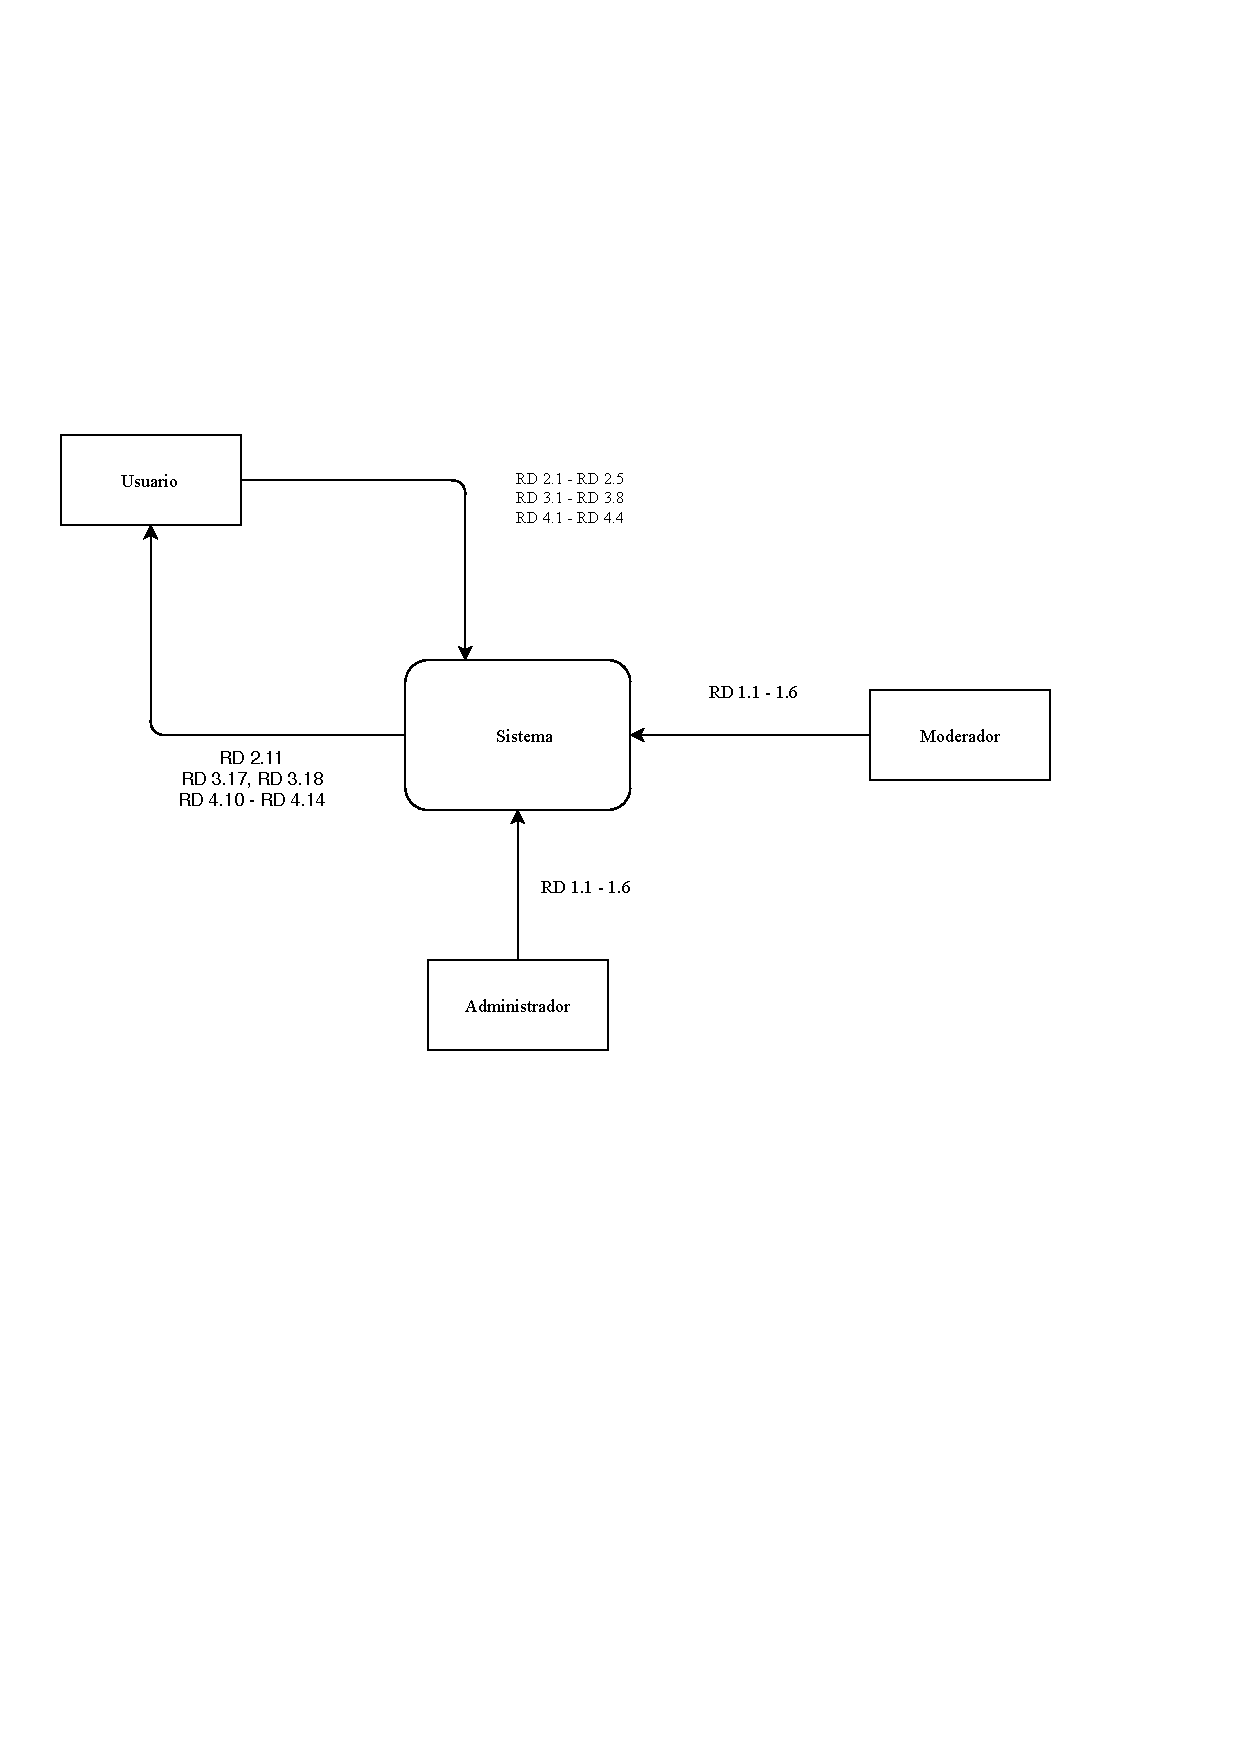
\includegraphics{diagramas/Caja_negra.pdf}
\end{figure}

\subsection{Esquema armazón}

\begin{figure}[H]
  \centering
  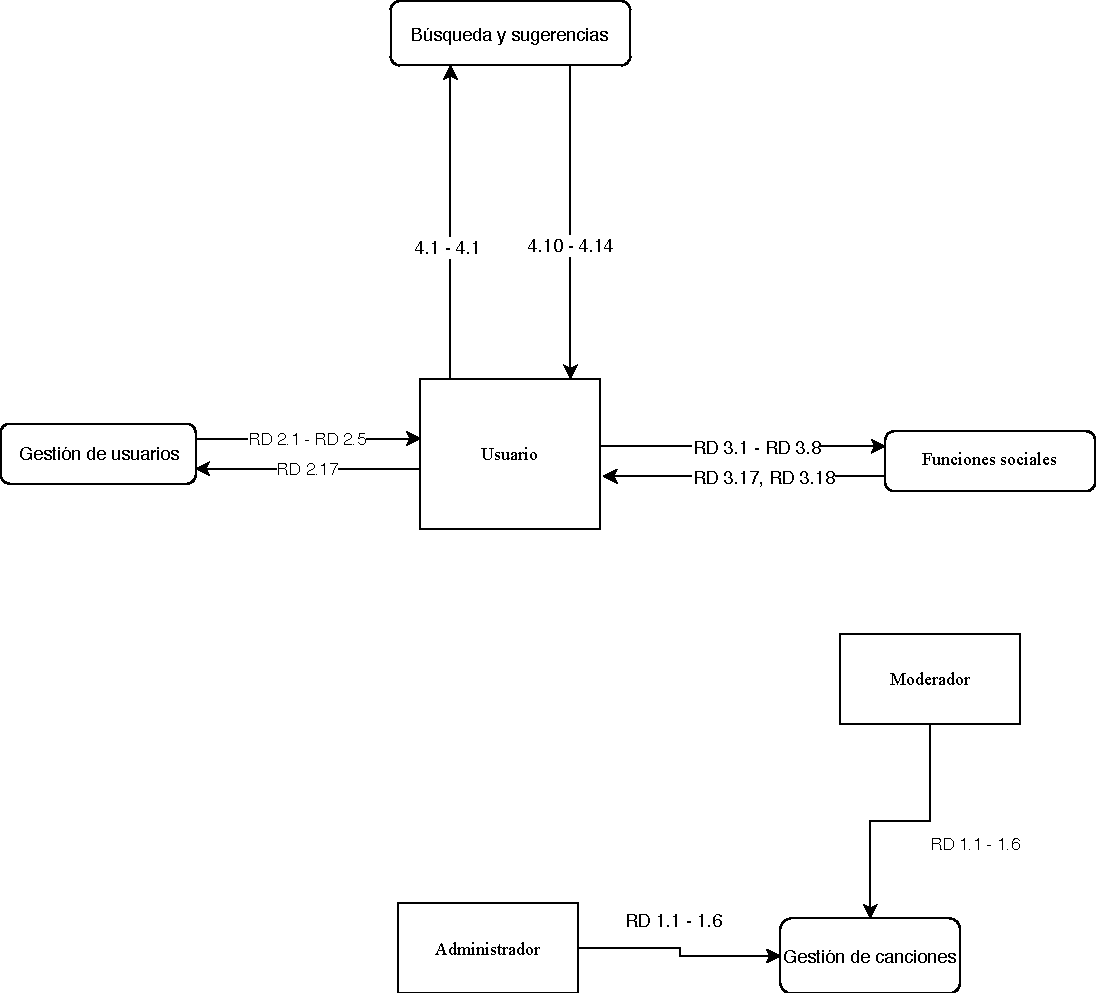
\includegraphics[scale=0.9]{diagramas/Esquema_armazon.pdf}
\end{figure}

\subsection{Refinamientos de los subsistemas}

\begin{figure}[H]
  \caption{Refinamiento del subsistema social}
  \centering
  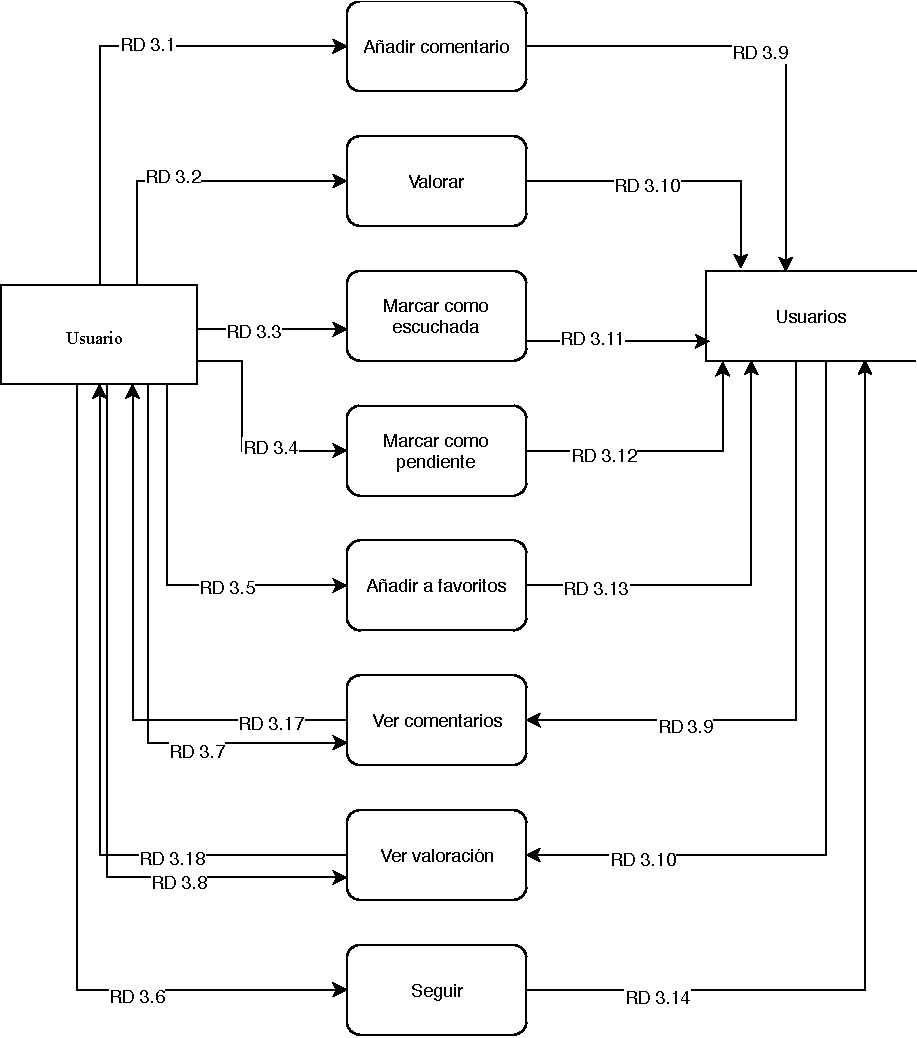
\includegraphics{diagramas/ref-social.pdf}
\end{figure}

\begin{figure}[H]
  \caption{Refinamiento del subsistema de búsquedas y sugerencias}
  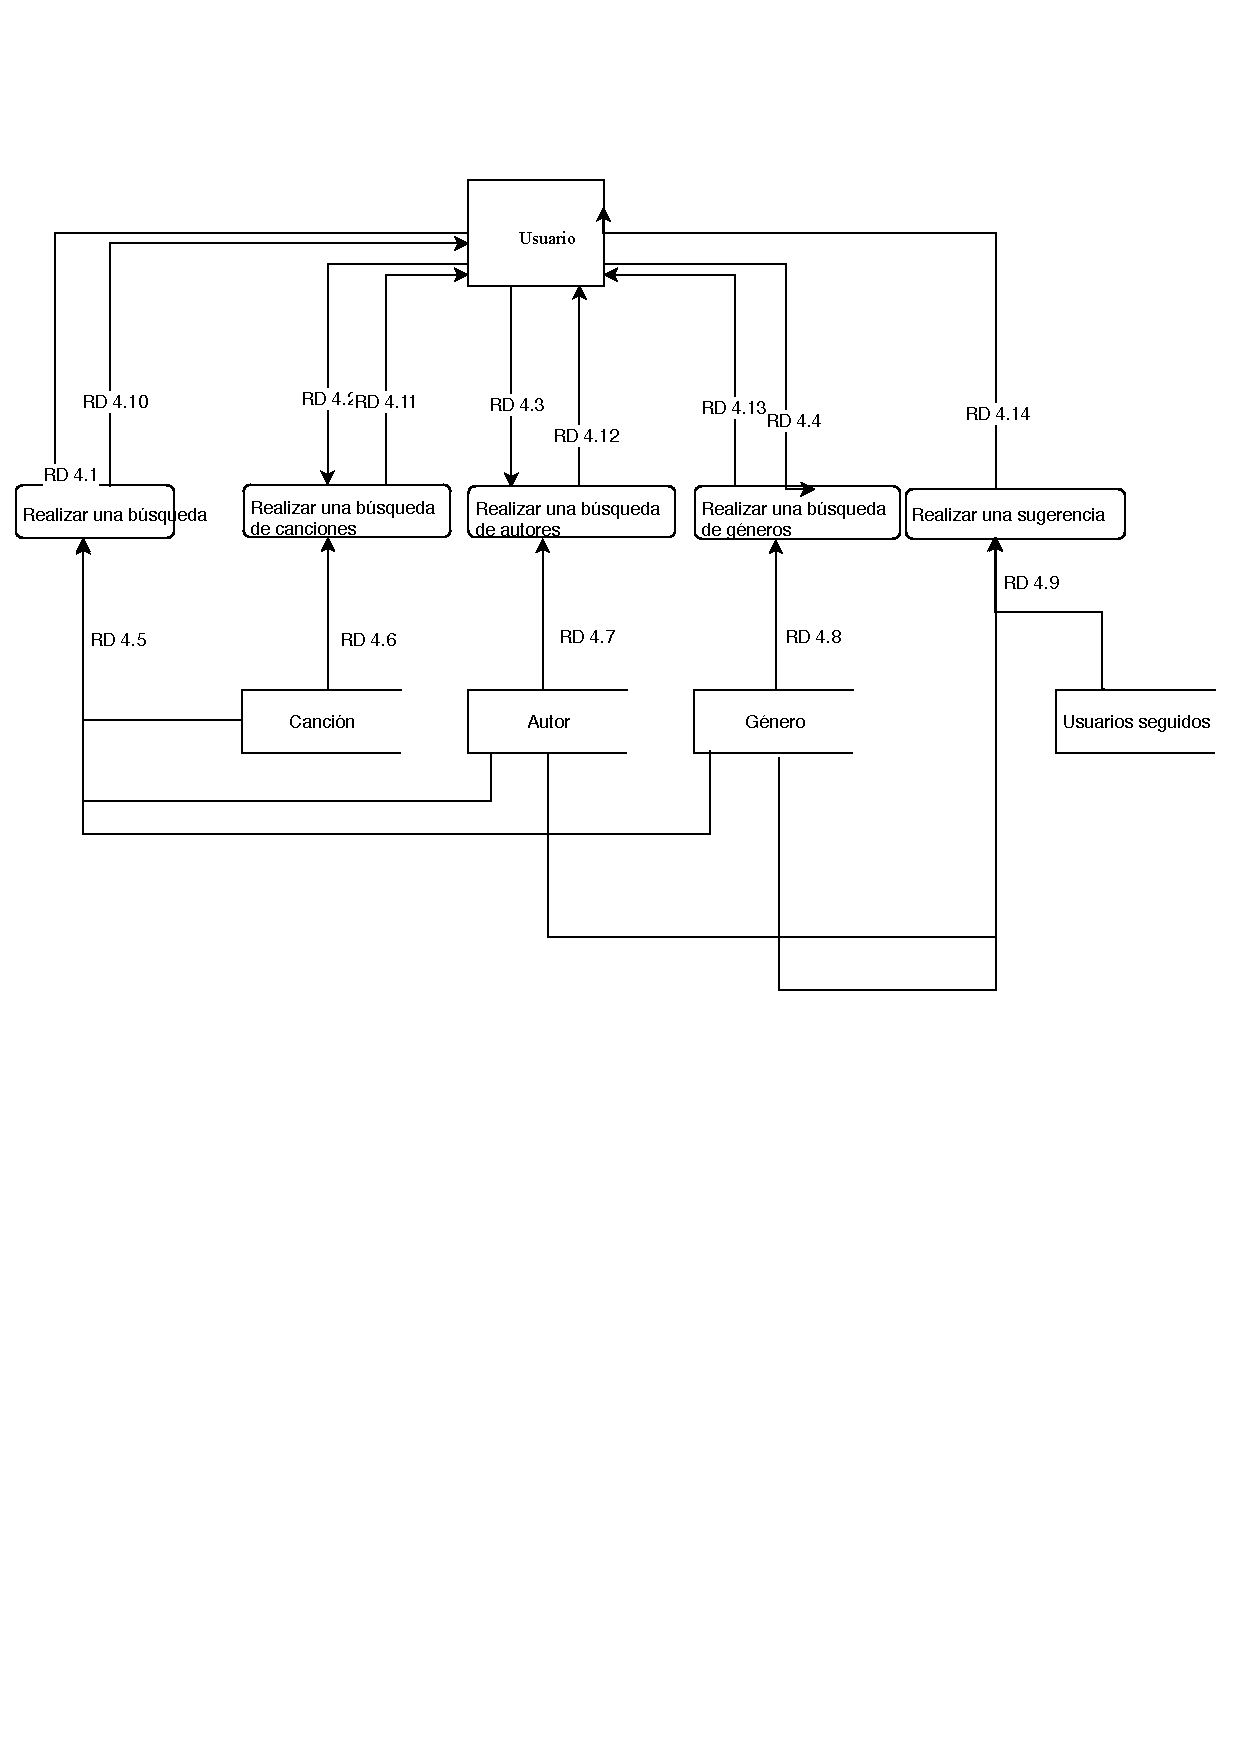
\includegraphics[scale=0.85]{diagramas/busqueda_refinamiento.pdf}
\end{figure}

\subsection{Esquemas externos}

\begin{figure}[H]
  \caption{Esquemas externos del subsistema social}
  \centering
  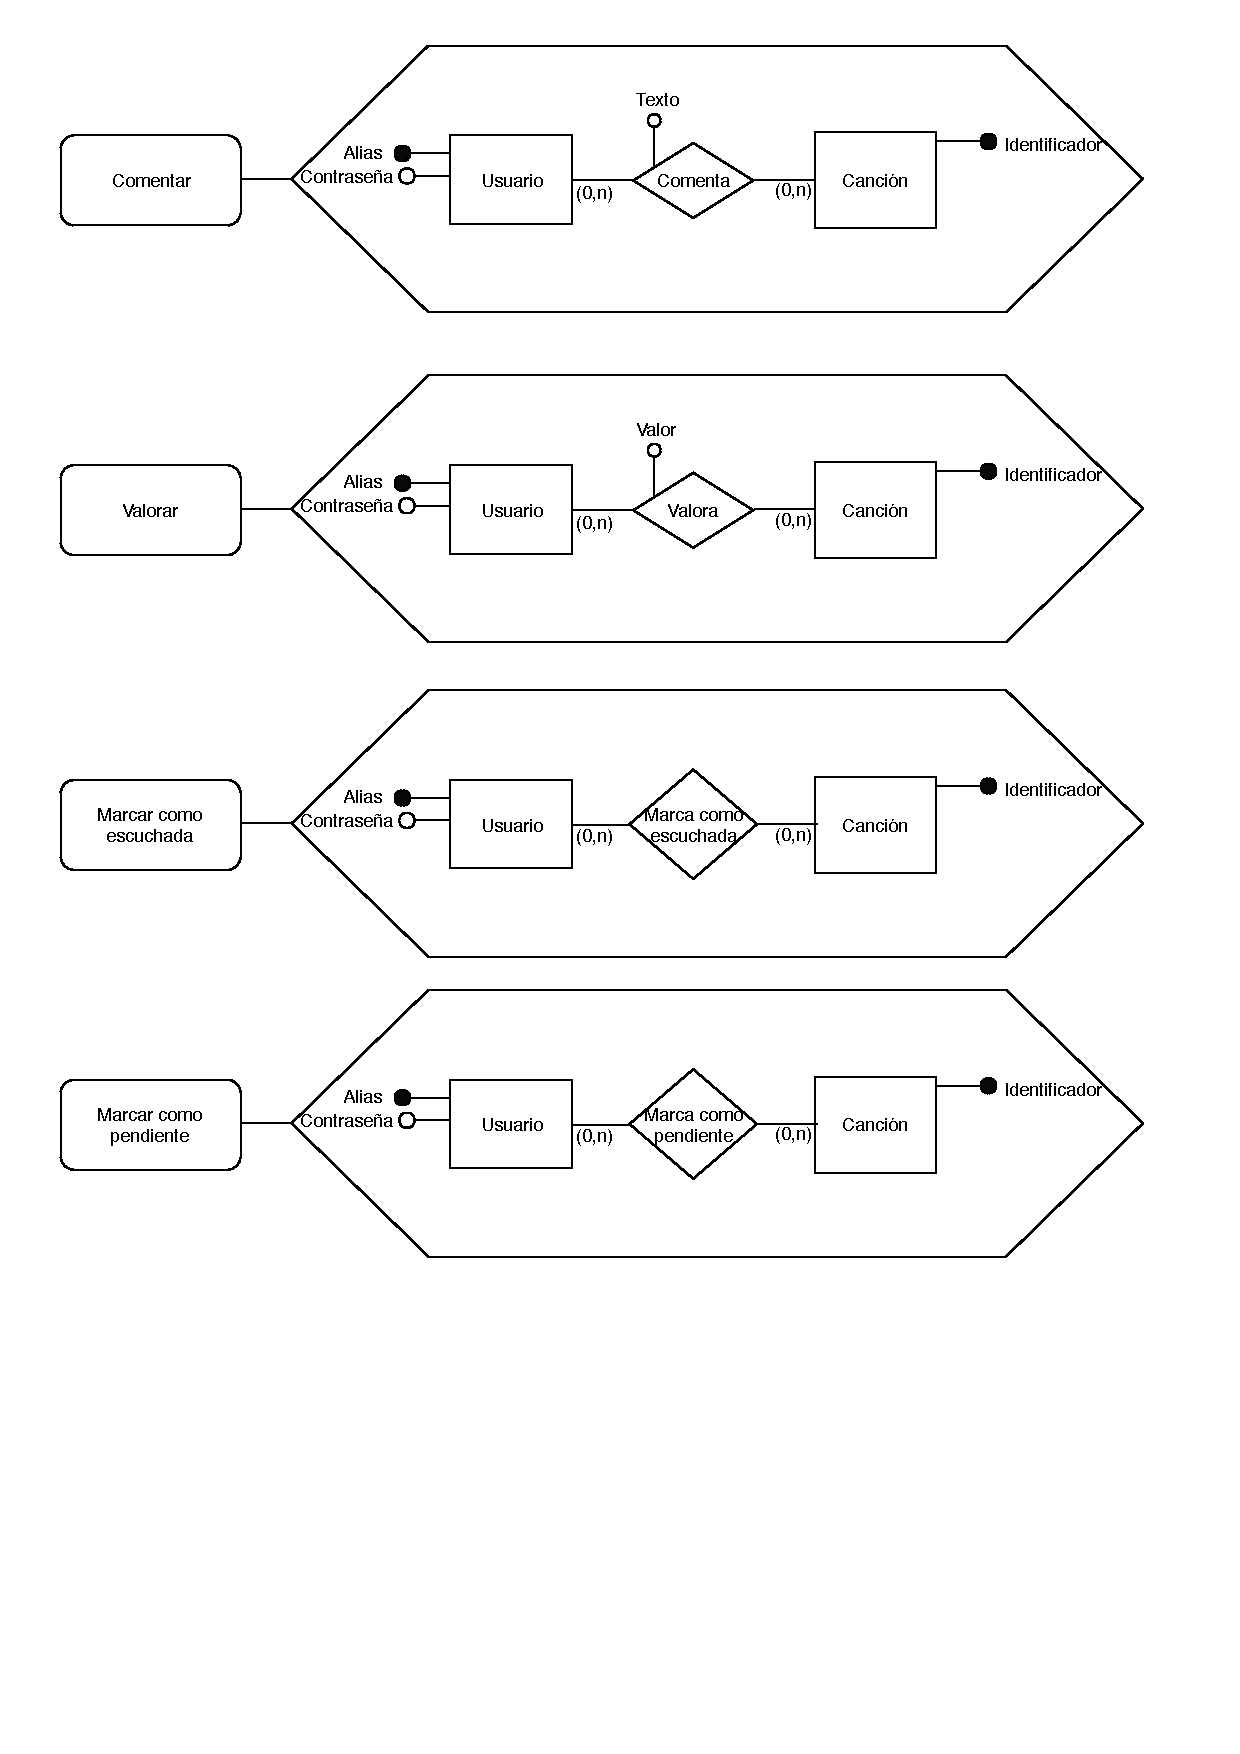
\includegraphics[scale=0.6]{diagramas/Esq-ext-social.pdf}
\end{figure}

\begin{figure}[H]
  \caption{Esquemas externos del subsistema de búsquedas y sugerenicas}
  \centering
  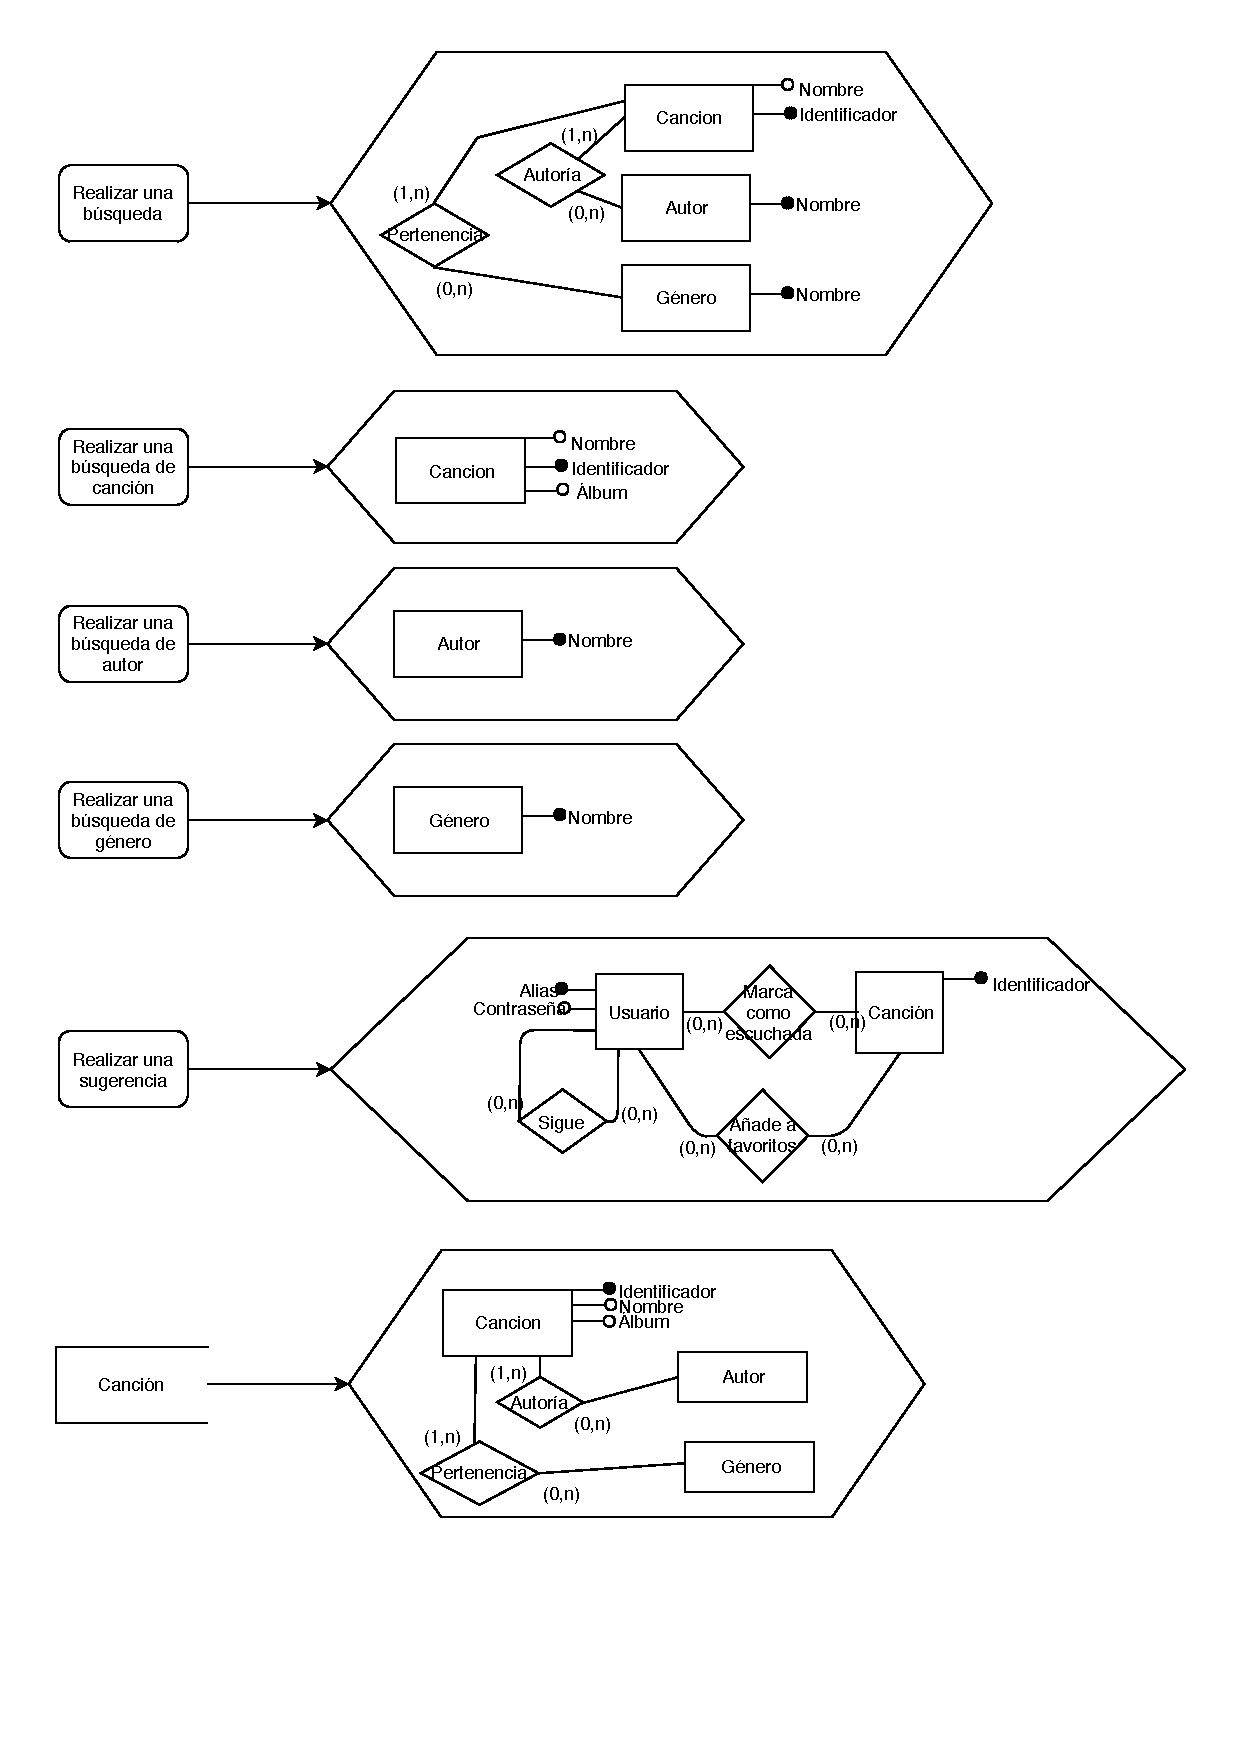
\includegraphics[scale=0.8]{diagramas/busqueda_esquema_externo.pdf}
\end{figure}

\subsection{Diagrama conceptual}

\begin{figure}[H]
  \caption{Diagrama conceptual del subsistema social}
  \centering
  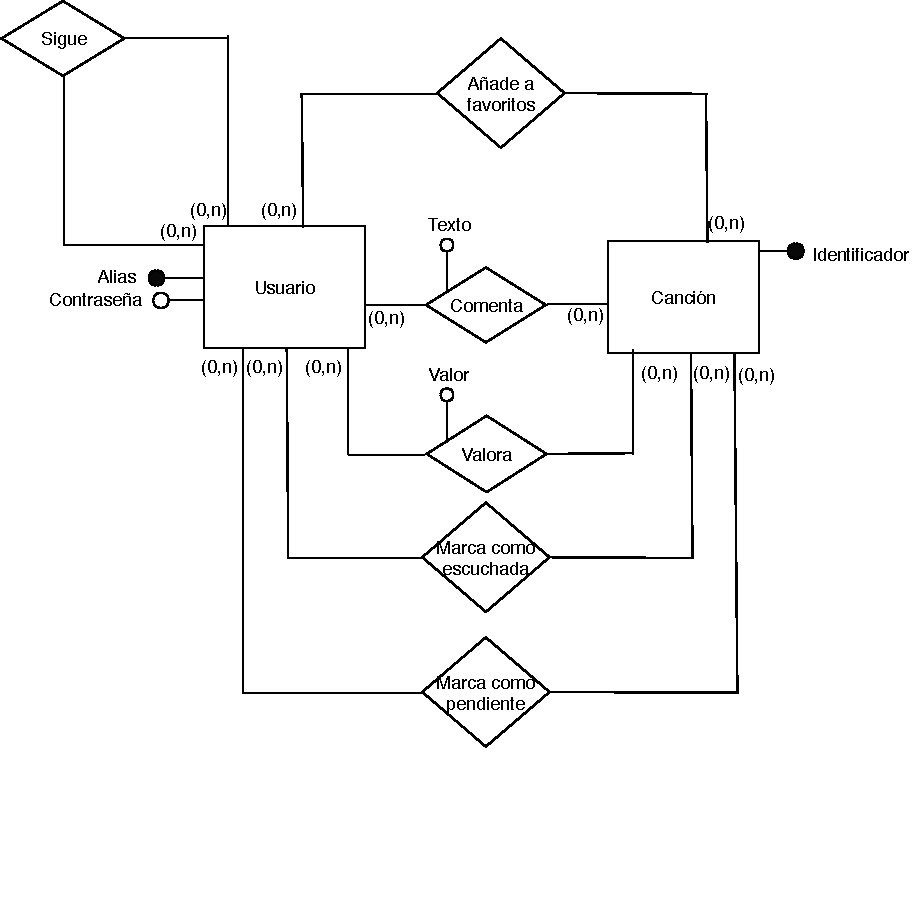
\includegraphics{diagramas/conceptual-social.pdf}
\end{figure}

\begin{figure}[H]
  \caption{Diagrama conceptual del subsistema de búsquedas y sugerencias}
  \centering
  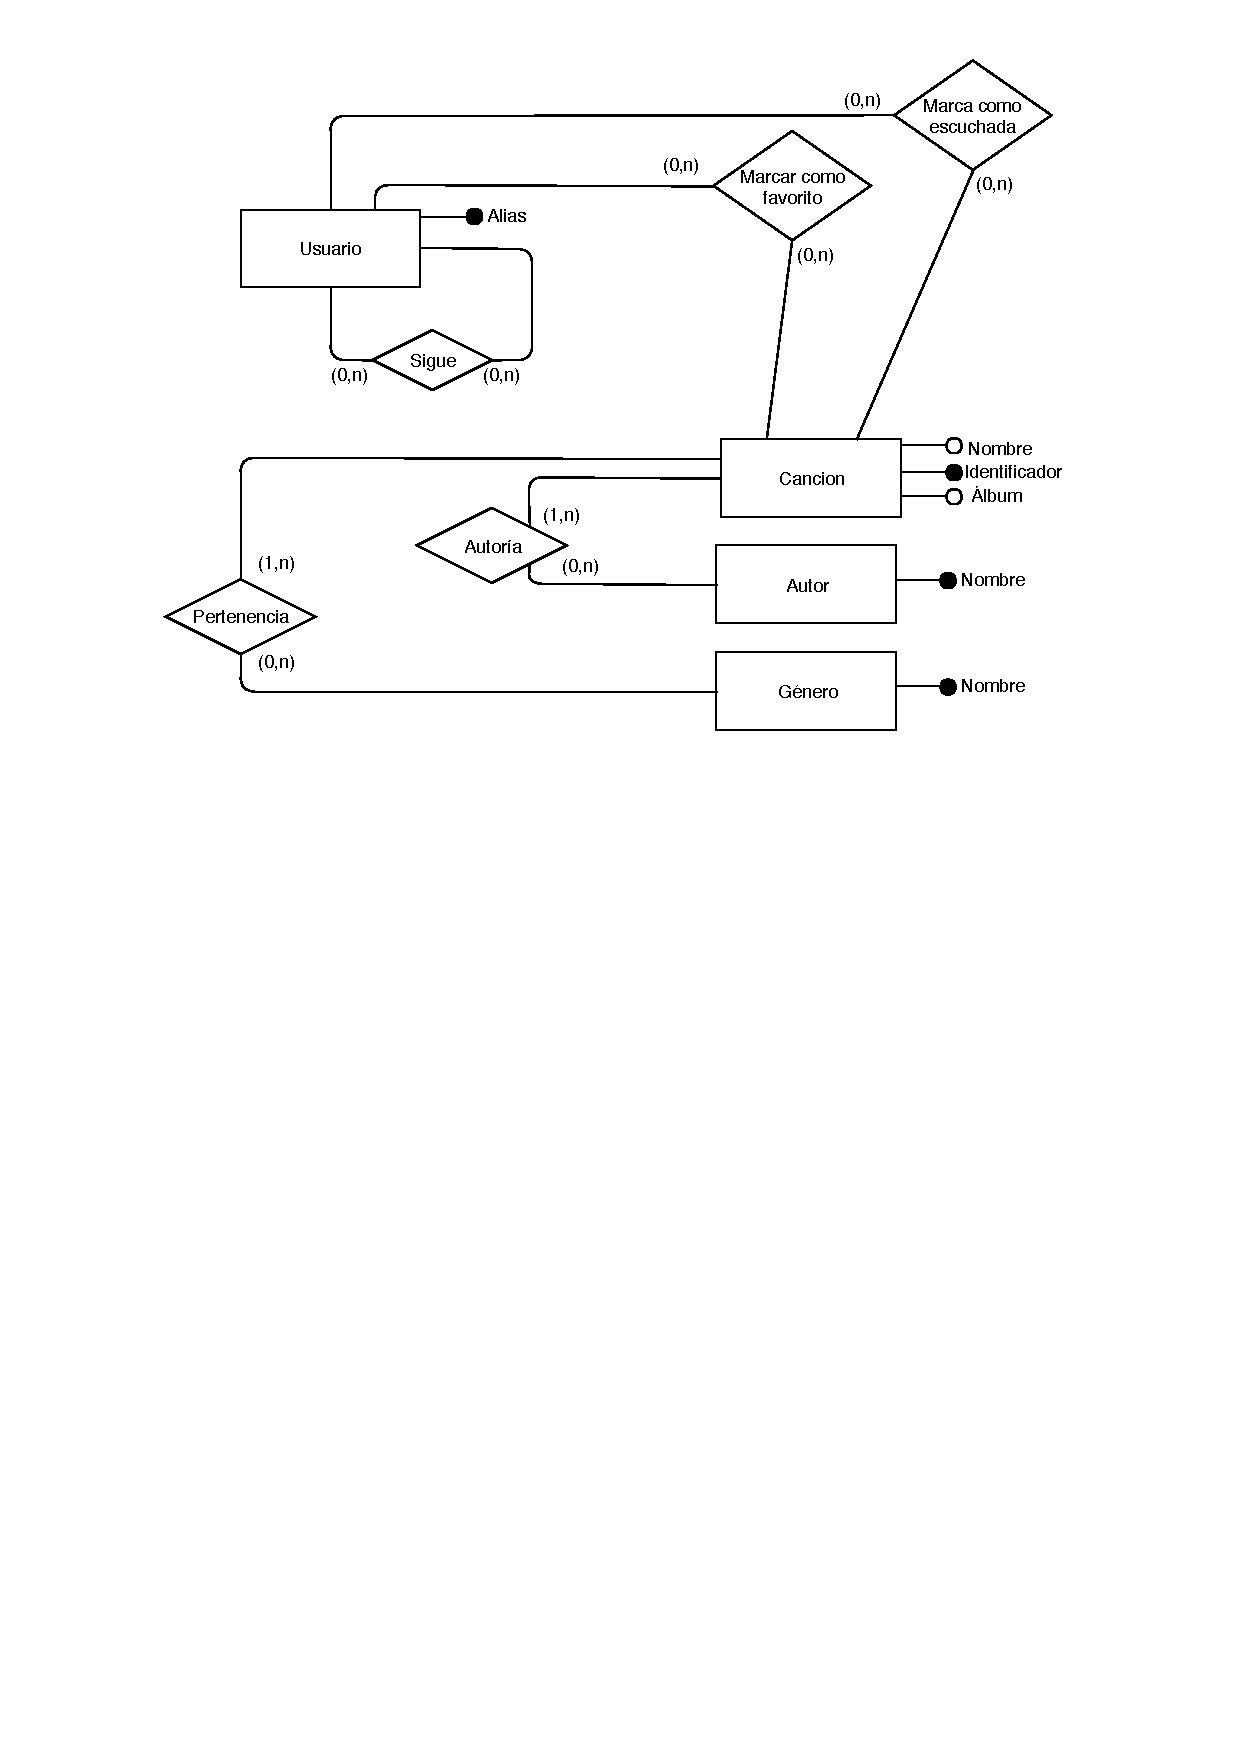
\includegraphics{diagramas/busqueda_modelo_conceptual.pdf}
\end{figure}

\subsection{Modelo entidad/relación}


\end{document}
